\chapter{MARCO TEÓRICO}
\section{Conceptos de lenguajes de programación}
``Los lenguajes de programación son notaciones que describen los cálculos a las personas y las máquinas. Nuestra percepción del mundo en que vivimos depende de los lenguajes de programación, ya que todo el software que se ejecuta en todas las computadoras se escribió en algún lenguaje de programación'' \cite[p. 1]{Aho2008}. Un lenguaje de programación es un lenguaje formal, que mediante un conjunto de instrucciones permite a un programador crear programas. El lenguaje de programación es un sistema estructurado de comunicación conformado por conjuntos de símbolos, palabras clave, reglas semánticas y sintácticas, las cuales sirven para el entendimiento entre un programador y una maquina.
\begin{itemize}
    \item \textbf{Palabra clave.} En los lenguajes de programacion existen palabras clave. Estas palabras no se pueden ser utilizadas para ningun otro proposito.
    \item \textbf{Funciones.} Tambien conocidos como subprogramas, procedimientos o metodos, las funciones son segmentos de codigo separado del bloque principal.
    \item \textbf{Tipos de datos.} En los lenguajes de programacion los tipos de datos son variados, los tipos de datos son atributos que indica la clase de dato que se va manejar. Los datos mas comunes son: Numeros enteros, numeros en coma flotante y cadenas.
    \item \textbf{Operadores.} Son simbolos que indican como manipular los operandos. Los operadores mas comunes son: Aritmeticos, relacionales, asignacion, logicos y tratamiento de bits.
    \item \textbf{Comentarios.} Son secuencias de caracteres que sirven para realizar anotaciones en el codigo fuente.
\end{itemize}

\section{Conceptos de ofuscación de código fuente}
\subsection{Código fuente}
En informática, se denomina código fuente a la conjunto de lineas de texto que escritas por un programador. Estas lineas de texto representan instrucciones en un lenguaje de programación. Las instrucciones representan los pasos que debe seguir la computadora para la ejecución de un programa específico. El código fuente no es directamente ejecutable por la computadora, este debe ser traducido a otro lenguaje de modo que la computadora pueda interpretarlo. En la traducción se usan compiladores, ensambladores, interpretes y otros.

\subsection{Ofuscación de código fuente}
En computación, la ofuscación de código fuente se refiere al acto de realizar cambios no destructivos en código fuente de un programa. Es decir, se alteran las instrucciones del código fuente manteniendo su funcionamiento original, la ofuscación de un programa se realiza para dificultar su entendimiento, también puede ser utilizado para ocultar la similitud con el programa original. Un ejemplo se muestra en la figura \ref{obfuscationSC}.


\begin{figure}[!h]
\centering
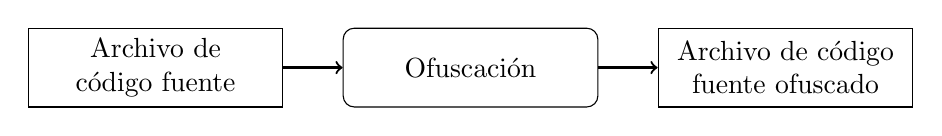
\begin{tikzpicture}[scale=1,
input_output/.style ={rectangle, minimum width=1cm, minimum height=1cm,text centered, text width=3cm, draw=black},
algorithm/.style={rectangle, rounded corners, minimum width=3cm, minimum height=1cm,text centered, text width=3cm, draw=black},
arrow/.style={thick,->,},
]
\node[input_output] (n0) at (1,1) {Archivo de código fuente};
\node[algorithm] (n1) at (5,1) {Ofuscación};
\node[input_output] (n2) at (9,1) {Archivo de código fuente ofuscado};
\draw [arrow] (n0.east) to (n1.west);
\draw [arrow] (n1.east) to (n2.west);
\end{tikzpicture}
\caption{Ofuscación de código fuente}
Fuente: Elaboración propia.
\label{obfuscationSC}
\end{figure}


Una definición formal se encuentra en \cite{Collberg1997} que define a la ofuscación de código fuente de la siguiente manera: Dado un programa $P$, y el programa transformado ${P}'$. Se define a $T$ como la transformación de ofuscación como $P\overset{T}{\rightarrow}{P}'$, donde requiere que $P$ y ${P}'$ mantengan el mismo comportamiento observacional, Ademas si $P$ no puede terminar o termina con errores, entonces ${P}'$ puede terminar o no, y ${P}'$ debe terminar si ${P}$ termina.

\subsection{Métodos de ofuscación de código fuente}
\cite{Novak2019} Explica que existen muchos métodos de ofuscación son utilizados para ocultar la similitud, a su vez menciona que en un estudio de 72 artículos se identificaron 25 métodos de ofuscación, y de estos se especificaron 16 métodos distintos. Existen muchos métodos para la ofuscación, a continuación se presentan los métodos mas importantes, cada método tiene su ejemplo de ofuscación en el lenguaje de programacion Python.

\begin{itemize}
    \item \cite{article3} Mencionan cambios en el formato del código. Como la agregación o eliminación de: Espacios en blanco, sangrías y saltos de linea. El ejemplo se muestra en los programas \ref{lst:obfuscation1_1} y \ref{lst:obfuscation1_2}.
    \lstinputlisting[caption={Cambio del formato del código, original},label={lst:obfuscation1_1}, language=Python]{programs/obfuscation/obfuscation1_1.py}
    \lstinputlisting[caption={Cambio del formato del código, modificado},label={lst:obfuscation1_2}, language=Python]{programs/obfuscation/obfuscation1_2.py}

    \item \cite{article3} Mencionan cambios en los comentarios del código. Como la agregación, modificación o eliminación de los comentarios. El ejemplo se muestra en los programas \ref{lst:obfuscation2_1} y \ref{lst:obfuscation2_2}.
    \lstinputlisting[caption={Cambios de comentarios, original},label={lst:obfuscation2_1}, language=Python]{programs/obfuscation/obfuscation2_1.py}
    \lstinputlisting[caption={Cambios de comentarios, modificado},label={lst:obfuscation2_2}, language=Python]{programs/obfuscation/obfuscation2_2.py}

    \item \cite{Zoran2012} y \cite{donaldson1981plagiarism} Mencionan el cambio de los nombres de los identificadores. Es decir, cambios en los nombres de variables, nombres de constantes, nombres de funciones, nombres de clases, etc. El ejemplo se  muestra en los programas \ref{lst:obfuscation3_1} y \ref{lst:obfuscation3_2}.
    \lstinputlisting[caption={Cambio en los nombres de las variables, original},label={lst:obfuscation3_1}, language=Python]{programs/obfuscation/obfuscation3_1.py}
    \lstinputlisting[caption={Cambio en los nombres de las variables, modificado},label={lst:obfuscation3_2}, language=Python]{programs/obfuscation/obfuscation3_2.py}

    \item \cite{donaldson1981plagiarism} Menciona cambios en el orden en las declaraciones de las variables. El ejemplo se muestra en los programas \ref{lst:obfuscation4_1} y \ref{lst:obfuscation4_2}.
    \lstinputlisting[caption={Cambio en el orden de declaraciones de variables, original},label={lst:obfuscation4_1}, language=Python]{programs/obfuscation/obfuscation4_1.py}
    \lstinputlisting[caption={Cambio en el orden de declaraciones de variables, modificado},label={lst:obfuscation4_2}, language=Python]{programs/obfuscation/obfuscation4_2.py}

    \item \cite{Grier1981} Menciona agregar lineas de código innecesarias. El ejemplo se muestra en los programas \ref{lst:obfuscation5_1} y \ref{lst:obfuscation5_2}.
    \lstinputlisting[caption={Agregar instrucciones innecesarias, original},label={lst:obfuscation5_1}, language=Python]{programs/obfuscation/obfuscation5_1.py}
    \lstinputlisting[caption={Agregar instrucciones innecesarias, modificado},label={lst:obfuscation5_2}, language=Python]{programs/obfuscation/obfuscation5_2.py}

    \item \cite{donaldson1981plagiarism} Menciona dividir una linea de código en varias lineas. El ejemplo se muestra en los programas \ref{lst:obfuscation6_1} y \ref{lst:obfuscation6_2}.
    \lstinputlisting[caption={Dividir una instruccion, original},label={lst:obfuscation6_1}, language=Python]{programs/obfuscation/obfuscation6_1.py}
    \lstinputlisting[caption={Dividir una instruccion, modificado},label={lst:obfuscation6_2}, language=Python]{programs/obfuscation/obfuscation6_2.py}

    \item \cite{WHALE1990131} Menciona el reemplazo de la llamada de un procedimiento por el procedimiento. El ejemplo se muestra en los programas \ref{lst:obfuscation7_1} y \ref{lst:obfuscation7_2}.
    \lstinputlisting[caption={Reemplazo de la llamada a un procedimiento, original},label={lst:obfuscation7_1}, language=Python]{programs/obfuscation/obfuscation7_1.py}
    \lstinputlisting[caption={Reemplazo de la llamada a un procedimiento, modificado},label={lst:obfuscation7_2}, language=Python]{programs/obfuscation/obfuscation7_2.py}

    \item \cite{WHALE1990131} Menciona el cambio de la especificación de una declaración. Cambios como: El cambio de las operaciones y el operando, cambio en los tipos de datos. El ejemplo se muestra en los programas \ref{lst:obfuscation8_1} y \ref{lst:obfuscation8_2}.
    \lstinputlisting[caption={Cambio de operaciones y operandos, original},label={lst:obfuscation8_1}, language=Python]{programs/obfuscation/obfuscation8_1.py}
    \lstinputlisting[caption={Cambio de operaciones y operandos, modificado},label={lst:obfuscation8_2}, language=Python]{programs/obfuscation/obfuscation8_2.py}

    \item \cite{article3} Mencionan el cambio de estructuras de control por sus equivalentes. El reemplazo por equivalentes de estructuras repetitivas y condicionales, El ejemplo se muestra en los programas \ref{lst:obfuscation9_1} y \ref{lst:obfuscation9_2}.
    \lstinputlisting[caption={Cambio en la estructura repetitiva, original},label={lst:obfuscation9_1}, language=Python]{programs/obfuscation/obfuscation9_1.py}
    \lstinputlisting[caption={Cambio en la estructura repetitiva, modificado},label={lst:obfuscation9_2}, language=Python]{programs/obfuscation/obfuscation9_2.py}
    %\item \cite{Zoran2012} Mencionan la simplificación de código. El ejemplo se muestra en los programas \ref{lst:ofuscacion10_1} y \ref{lst:ofuscacion10_2}.
    %\lstinputlisting[caption={Simplificación de código, original},label={lst:ofuscacion10_1},language=Python]{programas/ofuscacion10_1.py}
    %\lstinputlisting[caption={Simplificación de código, modificado},label={lst:ofuscacion10_2},language=Python]{programas/ofuscacion10_2.py}
\end{itemize}

\cite{Bejarano2015} se refiere a los métodos como modificaciones y los divide en dos grupos:
\begin{itemize}
  \item \textbf{Cambios léxicos}. Estos no requieren un análisis gramatical o profundo conocimiento de programación para ser eficaces. Algunos ejemplos son: Eliminar comentarios, cambiar el formato de código fuente y cambiar los nombres de las variables.
  \item \textbf{Cambios estructurales}. Estos requiere conocimiento acerca de los lenguajes y técnicas de programación, estos cambios son altamente dependiente de el lenguaje de programación. Algunos ejemplos son: cambiar las estructuras de control, cambiar el orden de las sentencias, reemplazar la llamada a un procedimiento por el procedimiento, etc.
\end{itemize}

\subsection{Niveles de transformación}
Una de las investigación mas antiguas respecto a la ofuscación de código fuente, fue desarrollado por \cite{Faidhi1987} en su trabajo se refiere a los métodos utilizados para las ofuscación como transformaciones para ocultar la similitud. Explica que las transformaciones pueden ser divididas en niveles. Donde en niveles bajos se encuentran las transformaciones que realiza un programador novato para ocultar la similitud, y los niveles altos se encuentran las transformaciones que realiza un programador experto para ocultar la similitud. A continuación el detalle de estos niveles de transformación.
\begin{itemize}
  \item \textbf{Nivel 1.} Representa los cambios en los comentarios e indentación.
  \item \textbf{Nivel 2.} Representa cambios de nivel 1, y cambios en los identificadores.
  \item \textbf{Nivel 3.} Representa cambios de nivel 2, y cambios en las declaraciones. Es decir declarar constantes extras, cambiar las posiciones de las variables declaradas.
  \item \textbf{Nivel 4.} Representa cambios de nivel 3, y modificación de los métodos. Es decir cambios en las asignaciones de la funciones, cambiar de funciones por procedimientos, combinar y crear nuevas funciones.
  \item \textbf{Nivel 5.} Representa cambios de nivel 4. y cambios en las sentencias equivalentes. Es decir cambios en las estructuras de control equivalentes un for por un while.
  \item \textbf{Nivel 6.} Representa cambios de nivel 5, y cambios en las decisiones lógica. Es decir cambios en la expresiones.
\end{itemize}

\section{Detección de similitud de código fuente}
\cite{Novak2019} Realizo un estudio sistemático campo de la detección de plagio de código fuente, describe definiciones de plagio, herramientas para la detección de plagio, métricas de comparación, métodos de ofuscación, conjunto de datos para la comparación y algoritmos que utilizan las herramientas.
\subsection{Algoritmos para la detección de similitud}
En su estudio \cite{Novak2019} identifica algoritmos basados en estilo, basado en semántica, basado en texto, huellas dactilares, recuento de atributos, basado en estructura, coincidencia de cadenas, marca de agua, basado en historial, basado en XML, código compilado, basado en compresión, basado en grafos, basado en agrupamiento, basado en N-gramas y basado en árboles. También hace menciona que los enfoques basados en estructuras son mucho mejores y que la mayoría de las herramientas combinan más de un tipo de algoritmo. En el cuadro \ref{tiposDeAlgoritmos} se muestra detalles de estos como el primer y ultimo año de publicación de un algoritmo, el numero de artículos en los que aparecen y si utilizan la tokenización.

\begin{table}[H]
\centering
\begin{tabular}{|lllll|}
\hline
\multicolumn{1}{|c|}{Tipo de algoritmo}       & \multicolumn{1}{c|}{Ultimo año} & \multicolumn{1}{c|}{Primer año} & \multicolumn{1}{c|}{Nro. de artículos} & \multicolumn{1}{c|}{Tokenización} \\ \hline\hline
\multicolumn{1}{|l|}{Basado en estilo}        & \multicolumn{1}{c|}{2016}       & \multicolumn{1}{c|}{2011}       & \multicolumn{1}{c|}{5}                 & \multicolumn{1}{c|}{2}           \\ \hline
\multicolumn{1}{|l|}{Basado en semántica}     & \multicolumn{1}{c|}{2013}       & \multicolumn{1}{c|}{2010}       & \multicolumn{1}{c|}{7}                 & \multicolumn{1}{c|}{5}            \\ \hline
\multicolumn{1}{|l|}{Basado en texto}         & \multicolumn{1}{c|}{2016}       & \multicolumn{1}{c|}{1996}       & \multicolumn{1}{c|}{9}                 & \multicolumn{1}{c|}{5}           \\ \hline
\multicolumn{1}{|l|}{Huellas dactilares}      & \multicolumn{1}{c|}{2015}       & \multicolumn{1}{c|}{2005}       & \multicolumn{1}{c|}{11}                & \multicolumn{1}{c|}{4}            \\ \hline
\multicolumn{1}{|l|}{Recuento de atributos}   & \multicolumn{1}{c|}{2015}       & \multicolumn{1}{c|}{1980}       & \multicolumn{1}{c|}{25}                & \multicolumn{1}{c|}{6}            \\ \hline
\multicolumn{1}{|l|}{Basado en estructura}    & \multicolumn{1}{c|}{2016}       & \multicolumn{1}{c|}{1980}       & \multicolumn{1}{c|}{25}                & \multicolumn{1}{c|}{13}           \\ \hline
\multicolumn{1}{|l|}{Coincidencia de cadenas} & \multicolumn{1}{c|}{2016}       & \multicolumn{1}{c|}{1981}       & \multicolumn{1}{c|}{26}                & \multicolumn{1}{c|}{17}           \\ \hline\hline
\multicolumn{5}{|c|}{Nuevas categorías identificadas}                                                                                                                    \\ \hline\hline
\multicolumn{1}{|l|}{Marca de agua}           & \multicolumn{1}{c|}{2013}       & \multicolumn{1}{c|}{2005}       & \multicolumn{1}{c|}{2}                 & \multicolumn{1}{c|}{0}            \\ \hline
\multicolumn{1}{|l|}{Basado en historial}     & \multicolumn{1}{c|}{2016}       & \multicolumn{1}{c|}{2013}       & \multicolumn{1}{c|}{2}                 & \multicolumn{1}{c|}{0}            \\ \hline
\multicolumn{1}{|l|}{Basado en XML}           & \multicolumn{1}{c|}{2012}       & \multicolumn{1}{c|}{2010}       & \multicolumn{1}{c|}{3}                 & \multicolumn{1}{c|}{2}            \\ \hline
\multicolumn{1}{|l|}{Código compilado}        & \multicolumn{1}{c|}{2015}       & \multicolumn{1}{c|}{2006}       & \multicolumn{1}{c|}{5}                 & \multicolumn{1}{c|}{2}            \\ \hline
\multicolumn{1}{|l|}{Basado en compresión}    & \multicolumn{1}{c|}{2010}       & \multicolumn{1}{c|}{2004}       & \multicolumn{1}{c|}{6}                 & \multicolumn{1}{c|}{5}            \\ \hline
\multicolumn{1}{|l|}{Basado en grafos}        & \multicolumn{1}{c|}{2015}       & \multicolumn{1}{c|}{2005}       & \multicolumn{1}{c|}{10}                & \multicolumn{1}{c|}{2}            \\ \hline
\multicolumn{1}{|l|}{Basado en agrupamiento}  & \multicolumn{1}{c|}{2015}       & \multicolumn{1}{c|}{2005}       & \multicolumn{1}{c|}{11}                & \multicolumn{1}{c|}{7}            \\ \hline
\multicolumn{1}{|l|}{Basado en N-gramas}      & \multicolumn{1}{c|}{2016}       & \multicolumn{1}{c|}{2006}       & \multicolumn{1}{c|}{15}                & \multicolumn{1}{c|}{9}            \\ \hline
\multicolumn{1}{|l|}{Basado en árboles}       & \multicolumn{1}{c|}{2015}       & \multicolumn{1}{c|}{1988}       & \multicolumn{1}{c|}{24}                & \multicolumn{1}{c|}{8}            \\ \hline
\end{tabular}
\caption{Descripción general de los tipos de algoritmos}
Fuente: \cite{Novak2019}.
\label{tiposDeAlgoritmos}
\end{table}


\cite{Novak2019} Menciona que las tres herramientas principales para la detección de similitud, utilizan los algoritmos de Running-Karp-Rabin Greedy-String-Tiling (RKR GST), Winnowing-Fingerprint e implementaciones de tokenización.
%\subsection{Algoritmo Greedy-String-Tiling}
%\subsection{Algoritmo Winnowing-Fingerprint}
\subsection{Técnicas para la detección de similitud}
En su investigación \cite{Karnalim2019} clasifica las técnicas de detección de similitud en tres categorías: Basadas en conteo de atributos, basadas en estructuras y técnicas híbridas, a continuación se dará una breve descripción de cada una de ellas.

\begin{enumerate}
    \item \textbf{Técnicas basadas en conteo de atributos}. Estas técnicas determinan la similitud comparando las frecuencias de ocurrencias de los atributos del código fuente.
    \begin{enumerate}
      \item \textbf{Técnica estándar de conteo de atributos}. Esta técnica considera similares a dos archivos de código fuente si sus frecuencias de ocurrencias de sus atributos son las mismas. Como los operandos, operadores, espacios en blanco, numero de lineas, comentarios, declaraciones y otros. Uno de los primeros trabajos presentados fue por \cite{Ottenstein1976} en el cual utiliza cuatro métricas de software: El numero de operadores únicos, operandos únicos, operadores y operandos.
      \item \textbf{Técnicas basadas en recuperación de información}. Esta técnica se basa en realizar consultas especificas a una gran colección de documentos, Una consulta especifica es un segmento de código o archivo y la colección de documentos son los archivos cuyo contenido es similar al segmento o archivo inicial. Las técnicas basadas en recuperacion de la información (IR) se basan en el análisis semántico latente (LSA), y tiene como objetivo encontrar relaciones entre términos con la ayuda de descomposición en valores singulares. \cite{Cosma2012} utilizaron LSA para detectar similitud en trabajos realizados por estudiantes obteniendo buenos resultados, sugiriendo que la técnica puede mejorar el rendimiento en las herramientas de detección existente como JPLAG y Sherlock.
      \item \textbf{Técnicas basadas en agrupamiento}. En esta técnica los archivos de código fuente similares se muestran en grupos. \cite{Moussiades2005} fue el primero en utilizar la técnica que consiste en convertir los archivos en tokens y luego los agrupa utilizando un algoritmo de agrupación.
      \item \textbf{Técnicas basadas en clasificación}. Esta técnica aprende a buscar patrones de similitud de código fuente. \cite{Yasaswi2017} utilizo su algoritmo de clasificación para detectar la similitud ponderando las características, según el modelo de un lenguaje a nivel de caracteres, el cual se entreno en el código fuente del kernel de Linux.
      \item \textbf{Técnicas combinadas con conteo de atributos}. Varias técnicas de conteo de atributos se combinan con otras técnicas para mejorar la detección. En su trabajo \cite{Sidorov2017} combina técnicas basadas en recuperacion de información y clasificación, su técnica consiste en convertir los archivos en tokens de N-gramas sobre los cuales se realizara el análisis semántico latente.
    \end{enumerate}
    \item \textbf{Técnicas basadas en estructuras}. Estas técnicas comparan estructuras de dos códigos fuente para determinar su similitud.
    \begin{enumerate}
      \item \textbf{Técnicas basadas en emparejamiento de cadenas}. Esta técnica es de las mas antiguas y populares, En su investigación \cite{Wise1992} compara dos archivos de código fuente convirtiéndolos en cadenas de tokens, y para la medición de similitud usa el comando sdiff de UNIX.
      \item \textbf{Técnicas basadas en emparejamiento de arboles y grafos}. La comparación de arboles o grafos puede llegar a tomar un tiempo considerable, por lo cual esta técnica suele incorporar simplificaciones que reduzcan el tiempo. En su investigación \cite{Song2015} calcula la similitud de código fuente de dos programas. Utilizando la información sintáctica del código fuente expresado como un árbol de análisis, la similitud sintáctica entre dos programas se calcula mediante un núcleo de árbol de análisis.
    \end{enumerate}
    \item \textbf{Técnicas híbridas} Estas técnicas combinan las técnicas de recuento de atributos, técnicas basadas en estructuras y otras. con el fin de mejorar la eficacia y eficiencia, para la comparación de similitud entre códigos fuente.
\end{enumerate}

\subsection{Herramientas para la detección de similitud}

\cite{Novak2019} describe cuatro características de cinco herramientas que son consideradas las más importantes, en el cuadro \ref{descripcionHerramientas} se muestran las características como: las menciones en artículos, código abierto, interfaz grafica (GUI), sin conexión a internet y el sitio web.

\begin{table}[H]
\centering
\begin{tabular}{|c||c|c|c|c|c|}
\hline
Herramienta      & Menciones & Código abierto & GUI & offline & Sitio web \\ \hline\hline
JPLAG        & 43                & Si             & Si  & Si                      & \href{https://jplag.ipd.kit.edu}{jplag.ipd.kit.edu} \\ \hline
MOSS          & 38                & No             & Si  & No                      & \href{https://theory.stanford.edu/~aiken/moss/}{theory.stanford.edu} \\ \hline
Sherlock & 9                 & Si             & Si  & Si                      & \href{http://warwick.ac.uk/iasgroup/software/sherlock}{warwick.ac.uk}  \\ \hline
Plaggie             & 7                 & Si             & Si  & Si                      &  \href{https://www.cs.hut.fi/Software/Plaggie}{www.cs.hut.fi} \\ \hline
SIM            & 6                 & Si             & No  & Si                      &  \href{https://dickgrune.com/Programs/similary_tester}{dickgrune.com} \\ \hline
\end{tabular}
\caption{Descripción general de las características de las herramientas}
Fuente: \cite{Novak2019}.
\label{descripcionHerramientas}
\end{table}


\cite{Ragkhitwetsagul2018} Realizo un estudio sobre métodos y herramientas para la detección de similitud, en el cual identifica las medidas de similitud que utilizan las cinco herramientas mas populares. En el cuadro \ref{descripcionHerramientasMedida} se muestra los detalles de las medidas de similitud que utilizan las cinco herramientas más populares.

\begin{table}[H]
\centering
\begin{tabular}{|r||l|}
\hline
Herramientas & Medida de similitud utilizadas \\ \hline\hline
JPLAG       & Tokens y Greedy-String-Tiling \\ \hline
MOSS        & Winnowing-Fingerprint \\ \hline
Sherlock    & Firmas Digitales  \\ \hline
Plaggie     & Token-Tiling  \\ \hline
SIM         & Alineamiento de cadenas  \\ \hline
\end{tabular}
\caption{Herramientas con sus medidas de similitud}
Fuente: \cite{Ragkhitwetsagul2018}.
\label{descripcionHerramientasMedida}
\end{table}


\subsubsection{JPLAG}
\cite{Prechelt2003} Explica que JPLAG es un servicio web que encuentra programas similares entre un conjunto de programas. Se ha utilizado con éxito para detectar plagio entre los envíos de programas Java de los estudiantes. Está disponible para los lenguajes C, C++ y Scheme, su algoritmo de comparación, se basa en uno conocido como Running-Rabin-Karp Greedy-String-Tiling. \cite{Cheers2021} Explica que JPLAG opera aplicando un algoritmo Token-Tiling para cubrir un archivo de código fuente con tokens extraídos de otro. Si dos archivos fuente tienen un alto grado de cobertura, pueden considerarse similares y, por lo tanto, candidatos a plagio. Primero, los archivos de código fuente se convierten en un flujo de tokens. JPlag utiliza su propio conjunto de tokens que abstraen los tokens de lenguaje estándar para evitar hacer coincidir el mismo token con diferentes significados. En segundo lugar, los tokens extraídos se comparan entre archivos para determinar la similitud mediante el algoritmo Running-Karp-Rabin Greedy-String-Tiling, donde los tokens de un archivo se superponen a los de otro dentro de una tolerancia de desajuste. La similitud del programa se evalúa como el porcentaje de tokens de un programa que se pueden colocar sobre otro programa.
\subsubsection{MOSS}
\cite{Hage2010} Explica que MOSS es un Software creado por el profesor Alex Aiken en la universidad de Stanford, siendo el primer servicio que inició en la web, una referencia a nivel mundial. MOSS permite comparar hasta 250 archivos en 25 lenguajes de programación. \cite{Pachon2019} Explica que MOSS no tiene licencia como software libre, el uso de MOSS dentro del ambiente académico es gratuito y ofrecido desde un servidor de Stanford. Es difícil su configuración y tiene poca documentación.
\subsubsection{Sherlock}
\cite{Cheers2021} Explica que Sherlock implementa métodos de comparación de texto y tokenizados. En la herramienta, se compara la similitud de un par de programas 5 veces: en su forma original, se eliminan los espacios en blanco y los comentarios, como un archivo fuente tokenizado. En todos los casos, las comparaciones miden la similitud a través de la identificación de ejecuciones, una secuencia de líneas comunes a dos archivos que pueden verse interrumpidas por anomalías, como líneas adicionales.

\subsubsection{Plaggie}
 \cite{Ahtiainen2006} Explica que Plaggie es una aplicación Java independiente que se puede utilizar para comprobar ejercicios de programación Java. La funcionalidad de Plaggie es similar al servicio web JPlag publicado anteriormente, pero a diferencia de JPlag, Plaggie debe instalarse localmente y su código fuente está abierto. Aparentemente, Plaggie es el único motor de detección de plagio de código abierto para ejercicios de Java. \cite{Cheers2021} Explica que Plaggie es una herramienta que se afirma que funciona de manera similar a JPlag. Plaggie es una aplicación local en comparación con JPlag que originalmente se proporcionó como un servicio web, no existe una publicación que describa el funcionamiento de Plaggie, sin embargo, al examinar su código fuente, opera sobre representaciones tokenizadas de código que evalúan la similitud mediante Token-Tiling.
\subsubsection{SIM}
\cite{Cheers2021} Explica que SIM analiza programas en busca de similitud estructural mediante el uso de alineación de cadenas. Para dos programas, SIM primero analiza el código fuente creando un árbol de análisis. Luego, la herramienta representará los árboles de análisis como cadenas y los alineará insertando espacios para obtener una subsecuencia común máxima de sus tokens contenidos. La similitud de los programas se evalúa luego como el número de coincidencias.

\section{Conceptos de compiladores y tokens}
\subsection{Procesador de lenguaje}
Un procesador de lenguaje también llamado compilador. \cite{Aho2008} Explica que un procesador de lenguaje es un programa que puede leer un programa en un lenguaje y traducirlo en un programa equivalente en otro lenguaje. Una función importante del compilador es reportar cualquier error en el programa fuente que detecte durante el proceso de traducción.

\subsection{Análisis Léxico}
Una analizador lexico tambien es conocido como Lexer. \cite{Aho2008} Explica que la primera fase de un procesador de lenguaje, se le llama análisis léxico o escaneo. El analizador léxico lee el flujo de caracteres que componen el programa fuente y los agrupa en secuencias significativas, conocidas como lexemas. Para cada lexema, el analizador léxico produce como salida un token. Estos lexemas son los que pasaran a la siguiente fase, el análisis de la sintaxis. El analizador léxico ignora los espacios en blanco que separan los lexemas. \cite{catalan2010compiladores} Explica que esta fase consiste en leer el texto del código fuente carácter a carácter e ir generando los tokens. Estos tokens constituyen la entrada para el siguiente proceso de análisis. El agrupamiento de caracteres en tokens depende del lenguaje que se va a compilar. Es decir un lenguaje generalmente agrupara caracteres en tokens diferentes de otro lenguaje. Los tokens pueden ser de dos tipos, cadenas específicas como palabras reservadas, puntos y comas, etc., y no específicas, como identificadores, constantes y etiquetas. La diferencia entre ambos tipos de tokens radica en si ya son conocidos previamente o no. El analizador léxico irá ignorando las partes no esenciales para la siguiente fase, como pueden ser los espacios en blanco, los comentarios, etc., es decir, realiza la función de preprocesador en cierta medida. Por lo tanto, y resumiendo, el analizador léxico lee los caracteres que componen el texto del programa fuente y suministra tokens al analizador sintáctico.

\subsection{Tokenización de codigo fuente}
Los tokens son la unidad léxica basica, y los lexemas son las palabras de un codigo fuente. \cite{Aho2008} Explica los pasos para generar un token. Primeramente se leen los lexemas que componen del código fuente y los agrupa en categorías según su función, este proceso es llamado tokenización. En un lenguaje de programación un token puede tener en clases como: constantes, identificadores, operadores, palabras reservadas y separadores. Por ejemplo, suponga que un código fuente contiene la instrucción de asignación: $\id{posicion = inicial + velocidad * 60}$. En este ejemplo se ignora los espacios en blanco que separan a los lexemas, y los nombres de los lexemas =, + y * serán considerados como símbolos abstractos. A continuación se muestra el detalle de la tokenización de la instrucción:
\begin{itemize}
    \item $\id{posicion}$: es un lexema, se le asigna al token $[\id{id}, 1]$, en donde $\id{id}$ es un símbolo abstracto que representa la palabra identificador y 1 apunta a la entrada en la tabla de símbolos para $\id{posicion}$. La entrada en la tabla de símbolos para un identificador contiene información acerca de éste, como su nombre y tipo.
    \item $=$: El símbolo de asignación es un lexema, se al asigna el token $[=]$. Como este token no necesita un valor-atributo, se omite el segundo componente.
    \item $\id{inicial}$: es un lexema, se le asigna al token $[id, 2]$, en donde 2 apunta a la entrada en la tabla de símbolos para $\id{inicial}$.
    \item $+$: es un lexema, se le asigna al token $[+]$.
    \item $\id{velocidad}$: es un lexema, se le asigna al token $[id, 3]$, en donde 3 apunta a la entrada en la tabla de símbolos para $\id{velocidad}$.
    \item $*$: es un lexema, se le asigna al token $[*]$.
    \item $60$: es un lexema, se le asigna al token $[60]$.
\end{itemize}

\noindent Finalmente se obtiene los siguientes tokens: $[id, 1] [=] [id, 2] [+] [id, 3] [*] [60]$.

\section{Conceptos de grafos y algoritmos}
\subsection{Grafo direccionado}
En \cite{Cormen2009} encontramos la siguiente definición. Un grafo direccionado $G$ es un par $(V,E)$, donde $V$ es un conjunto finito y $E$ es una relación binaria en $V$. El conjunto V es llamado conjunto de vértices de $G$, y sus elementos son llamados vértices. El conjunto $E$ es llamado conjunto de aristas de $G$, y sus elementos son llamados aristas, como se muestra en la figura \ref{grafoDir}.

\begin{figure}[!h]
\centering
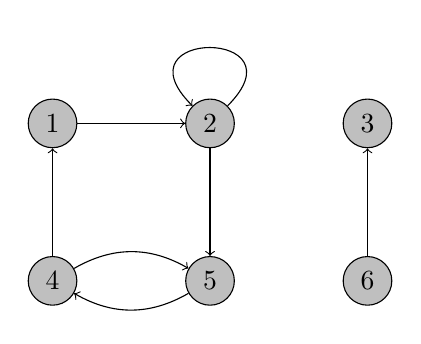
\begin{tikzpicture}[scale=1, vertex/.style = {circle,fill=gray!50,draw}, edge/.style = {->,thin}]
% vertex
\node[vertex] (n4) at (1,1) {4};
\node[vertex] (n5) at (3,1) {5};
\node[vertex] (n2) at (3,3) {2};
\node[vertex] (n1) at (1,3) {1};
\node[vertex] (n6) at (5,1) {6};
\node[vertex] (n3) at (5,3) {3};
%edges
\draw[edge] (n4) to (n1);
\draw[edge] (n1) to (n2);
\draw[edge] (n2) to (n5);
\draw[edge] (n6) to (n3);
\draw[edge] (n4) to[bend left] (n5);
\draw[edge] (n5) to[bend left] (n4);
\draw[edge] (n2) to[loop] (n2);
\end{tikzpicture}
\caption{Grafo direccionado}
Un grafo direccionado $G=(V,E)$, donde $V=\{1,2,3,4,5,6\}$ y $E=\{(1,2),(2,2),(2,4),(2,5),(4,1),(4,5),(4,5),(6,3)\}$. \\Fuente: \cite{Cormen2009}.
\label{grafoDir}
\end{figure}

\subsection{Grafo no direccionado}
En \cite{Cormen2009} encontramos la siguiente definición. Un grafo no direccionado $G=(V,E)$, el conjunto de aristas $E$ consiste en pares no ordenados de vértices, en lugar de pares ordenados. Es decir una arista es un conjunto $(u,v)$ donde $u,v \in V$ y $u \neq v$, considerando que $(u,v)$ y $(v,u)$ son la misma arista, como se muestra en la figura \ref{grafoNoDir}.

\begin{figure}[!h]
\centering
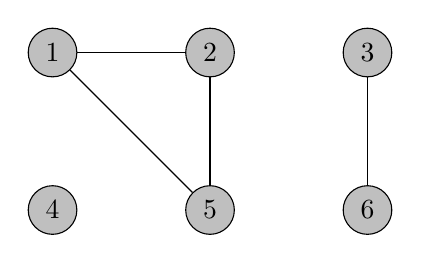
\begin{tikzpicture}[scale=1, vertex/.style = {circle,fill=gray!50,draw}, edge/.style = {-,thin}]
% vertex
\node[vertex] (n4) at (1,1) {4};
\node[vertex] (n5) at (3,1)  {5};
\node[vertex] (n2) at (3,3)  {2};
\node[vertex] (n1) at (1,3)  {1};
\node[vertex] (n6) at (5,1)  {6};
\node[vertex] (n3) at (5,3)  {3};
%edges
\draw[edge] (n1) to (n2);
\draw[edge] (n1) to (n5);
\draw[edge] (n2) to (n5);
\draw[edge] (n3) to (n6);
\end{tikzpicture}
\caption{Grafo no direccionado}
Un grafo no direccionado $G=(V,E)$, donde $V=\{1,2,3,4,5,6\}$ y $E=\{(1,2),(1,5),(2,5),(3,6)\}$.\\Fuente: \cite{Cormen2009}.
\label{grafoNoDir}
\end{figure}
\subsection{Grafo bipartito}
En \cite{Cormen2009} encontramos la siguiente definición. Un grafo bipartito es un grafo no direccionado $G=(V,E)$ en el cual $V$ puede ser particionado en dos conjuntos $V_1$ y $V_2$ talque $(u,v) \in E$ implica que $u \in V_1$ y $v \in V_2$ o $v \in V_1$ y $u \in V_2$. Es decir todas las aristas relacionan los conjuntos $V_1$ y $V_2$, como se muestra en la figura \ref{grafoBip}.
\begin{figure}[!h]
\centering
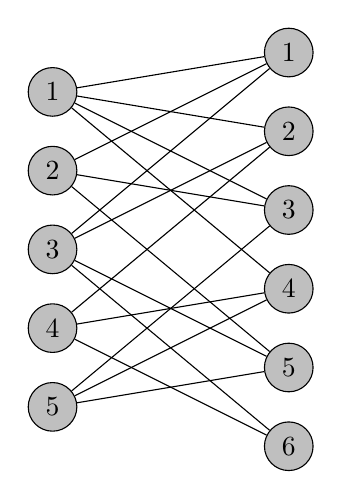
\begin{tikzpicture}[scale=1, vertex/.style = {circle,fill=gray!50,draw}, edge/.style = {-,thin}]
% vertex
\node[vertex] (n1) at (1,5.5) {1};
\node[vertex] (n2) at (1,4.5)  {2};
\node[vertex] (n3) at (1,3.5)  {3};
\node[vertex] (n4) at (1,2.5)  {4};
\node[vertex] (n5) at (1,1.5)  {5};
\node[vertex] (n6) at (4,6)  {1};
\node[vertex] (n7) at (4,5)  {2};
\node[vertex] (n8) at (4,4)  {3};
\node[vertex] (n9) at (4,3)  {4};
\node[vertex] (n10) at (4,2)  {5};
\node[vertex] (n11) at (4,1)  {6};
%edges
\draw[edge] (n1) to (n6);
\draw[edge] (n1) to (n7);
\draw[edge] (n1) to (n8);
\draw[edge] (n1) to (n9);
\draw[edge] (n2) to (n6);
\draw[edge] (n2) to (n8);
\draw[edge] (n2) to (n10);
\draw[edge] (n3) to (n6);
\draw[edge] (n3) to (n7);
\draw[edge] (n3) to (n10);
\draw[edge] (n3) to (n11);
\draw[edge] (n4) to (n7);
\draw[edge] (n4) to (n9);
\draw[edge] (n4) to (n11);
\draw[edge] (n5) to (n8);
\draw[edge] (n5) to (n9);
\draw[edge] (n5) to (n10);
\end{tikzpicture}
\caption{Grafo bipartito}
Un grafo bipartito con un numero impar de vértices.\\Fuente: \cite{Cormen2009}.
\label{grafoBip}
\end{figure}

\subsection{Lista de adyacencia}
\cite{Cormen2009} explica que la representación de grafo $G=(V,E)$ mediante listas de adyacencia, consiste en arreglo $Adj$ de $|V|$ listas, una para cada vértice en $V$. Para cada $u \in V$, la lista de adyacencia $Adj[u]$ contiene todos los vértices $v$ talque hay una arista $(u,v) \in E$. Es decir, $Adj[u]$ consiste en todos los vértices adyacentes de $u$ en $G$, un ejemplo se muestra en la figura \ref{listaAdy}.

\begin{figure}[!h]
\centering
\begin{tikzpicture}
\matrix (M) [matrix of nodes,
column sep=0pt,
row sep=0pt,
nodes={draw,fill=gray!50,minimum width=.5cm,outer sep=0pt,minimum
height=.5cm,anchor=center},
column 1/.style={minimum height=.8cm}]{
\mbox{} &[2mm] 2 & \mbox{} &[2mm] 5 & - &[2mm] & &[2mm] & \\
\mbox{} & 1 & \mbox{} & 5 & \mbox{} & 3 & \mbox{} & 4 & - \\
\mbox{} & 2 & \mbox{} & 4 & - & & & & \\
\mbox{} & 2 & \mbox{} & 5 & \mbox{} & 3 & - & & \\
\mbox{} & 4 & \mbox{} & 1 & \mbox{} & 2 & - & & \\
};
\foreach \i in {1,2,3,4,5}{
\path (M-\i-1) [late options={label=left:\i}];
\draw[->] (M-\i-1.center)--(M-\i-2.west);
\draw[->] (M-\i-3.center)--(M-\i-4.west);
}
\draw[->] (M-2-5.center)--(M-2-6.west);
\draw[->] (M-4-5.center)--(M-4-6.west);
\draw[->] (M-5-5.center)--(M-5-6.west);
\draw[->] (M-2-7.center)--(M-2-8.west);
\end{tikzpicture}
\caption{Ejemplo de la lista de adyacencia de un grafo}
Para un grafo $G=(V,E)$, donde $V = \{(1,2),(1,5),(2,1),(2,5),(2,3),(2,4),(3,2),(3,4),(4,2),(4,5),(4,3),(5,4),(5,1),(5,2)\}$. \\Fuente: \cite{Cormen2009}.
\label{listaAdy}
\end{figure}


\subsection{Búsqueda en profundidad}
La Busqueda en profundidad tambien es conocida por sus siglas en ingles como DFS. \cite{Halim2019} Explica que la búsqueda en profundidad, es un algoritmo sencillo para el recorrido de grafos. La búsqueda en profundidad comienza en un vértice de origen, recorre primero el grafo en profundidad, si durante el recorrido se encuentra con un vértice que tiene mas de un vecino, elige a uno de los vecinos no visitados y visitara su vértice. La búsqueda en profundidad repite este proceso en profundidad hasta que llega a un vértice terminal, cuando esto ocurre vuelve hacia atrás y explora otros vecinos todavía no visitados. Este comportamiento es de fácil implementación mediante recusión, un ejemplo de este recorrido se muestra en la figura \ref{ejemDfs}.

\begin{figure}[!h]
\centering
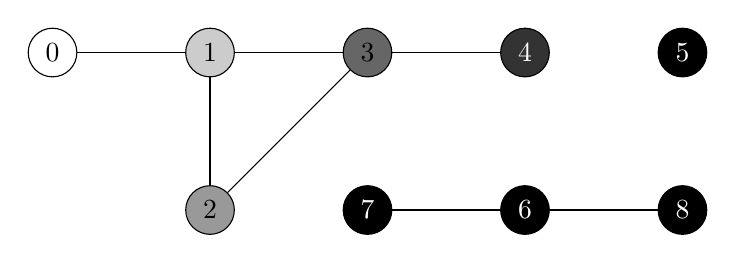
\begin{tikzpicture}[scale=1, label1/.style = {circle,fill=black!0,draw}, label2/.style = {circle,fill=black!20,draw}, label3/.style = {circle,fill=black!40,draw}, label4/.style = {circle,fill=black!60,draw}, label5/.style = {circle,fill=black!80,draw,text=white}, label6/.style = {circle,fill=black!100,draw, text=white}, edge/.style = {-,thin}]
% vertex
\node[label1] (n0) at (1,3)  {0};
\node[label2] (n1) at (3,3)  {1};
\node[label4] (n3) at (5,3)  {3};
\node[label5] (n4) at (7,3)  {4};
\node[label6] (n5) at (9,3)  {5};
\node[label3] (n2) at (3,1)  {2};
\node[label6] (n7) at (5,1)  {7};
\node[label6] (n6) at (7,1)  {6};
\node[label6] (n8) at (9,1)  {8};
%edges
\draw[edge] (n0) to (n1);
\draw[edge] (n1) to (n2);
\draw[edge] (n0) to (n1);
\draw[edge] (n1) to (n3);
\draw[edge] (n3) to (n4);
\draw[edge] (n3) to (n2);
\draw[edge] (n7) to (n6);
\draw[edge] (n6) to (n8);
\end{tikzpicture}
\caption{Ejemplo de búsqueda en profundidad}
Dado un grafo conexo no direccionado, se realiza la búsqueda en profundidad en $s=0$, obteniendo el siguiente recorrido $0 \rightarrow 1 \rightarrow 2 \rightarrow 3 \rightarrow 4$. \\Fuente: \cite{Halim2019}.
\label{ejemDfs}
\end{figure}

En la implementación de la búsqueda en profundidad. Para cada vértice $v \in V$, si $v$ fue visitado entonces $v.vis$ tendrá el valor de $\id{VISITED}$, caso contrario $v.vis$ tendrá el valor de $\id{UNVISITED}$. Es decir se marca con etiquetas a los vértices que fueron visitados o no visitados. La implementación en pseudocódigo del algoritmo se encuentra en $\proc{DFS}(G, s)$.

\begin{codebox}
\Procname{$\proc{DFS}(G, s)$}
\li For each vertex $v \in V$
\li \Do $v.vis \gets \id{UNVISITED}$ \End
\li $\proc{DFS-Visit}(G,s)$
\end{codebox}
\begin{codebox}
\Procname{$\proc{DFS-Visit}(G, u)$}
\li $u.vis \gets \id{VISITED}$
\li \For each vertex $v \in G.Adj[u]$
\li \Do \If $v.vis \isequal \id{UNVISITED}$
\li \Then $\proc{DFS-Visit}(G, v)$ \End \End
\end{codebox}

La complejidad temporal de la búsqueda en profundidad en un grafo que esta representado mediante una lista de adyacencia es $O(V+E)$.

\subsection{Búsqueda en anchura}
La busqueda en anchura tambien es conocida por sus siglas en ingles como BFS. \cite{Halim2019} explica que la busqueda en anchura es un algoritmo sencillo para el recorrido de grafos. Comenzando en un vértice de origen, recorre el grafo en anchura, visita todos los vértices vecinos del vértice de origen, seguido los vértices vecinos de los vecinos, y así sucesivamente. Es decir capa a capa. La búsqueda en anchura comienza con todos los vértices del grafo marcados como no visitados, inserta el vértice de origen $s$ en una cola $Q$ y marca a $s$ como visitado, luego mientras la cola no se encuentre vacía realiza el siguiente proceso: Quita el vértice $u$ que se encuentra en frente de la cola, para cada vértice vecino de $u$ que no haya sido visitado lo agrega a la cola y lo marca como visitado. Cuando la cola se encuentre vacía el algoritmo finaliza y se habrá recorrido todos los vértices del componente conexo que contiene a $s$, un ejemplo de este recorrido se muestra en la figura \ref{ejemBfs}.

\begin{figure}[!h]
\centering
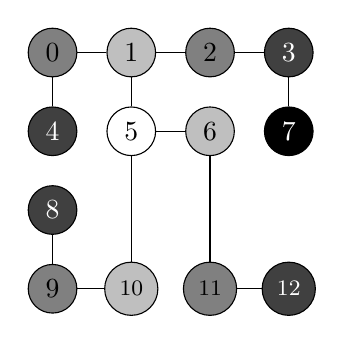
\begin{tikzpicture}[scale=1, label1/.style = {circle,fill=black!0,draw}, label2/.style = {circle,fill=black!25,draw}, label3/.style = {circle,fill=black!50,draw}, label4/.style = {circle,fill=black!75,draw, text=white}, label5/.style = {circle,fill=black!100,draw, text=white}, edge/.style = {-,thin}]
% vertex
\node[label1] (n5) at (2,3) {5};
\node[label2] (n10) at (2,1) {\footnotesize10};
\node[label2] (n1) at (2,4) {1};
\node[label2] (n6) at (3,3) {6};
\node[label3] (n9) at (1,1) {9};
\node[label3] (n11) at (3,1) {\footnotesize11};
\node[label3] (n0) at (1,4) {0};
\node[label3] (n2) at (3,4) {2};
\node[label4] (n8) at (1,2) {8};
\node[label4] (n4) at (1,3) {4};
\node[label4] (n12) at (4,1) {\footnotesize12};
\node[label4] (n3) at (4,4) {3};
\node[label5] (n7) at (4,3) {7};
%edges
\draw[edge] (n5) to (n1);
\draw[edge] (n5) to (n6);
\draw[edge] (n5) to (n10);
\draw[edge] (n1) to (n0);
\draw[edge] (n1) to (n2);
\draw[edge] (n10) to (n9);
\draw[edge] (n6) to (n11);
\draw[edge] (n0) to (n4);
\draw[edge] (n9) to (n8);
\draw[edge] (n2) to (n3);
\draw[edge] (n11) to (n12);
\draw[edge] (n3) to (n7);
\end{tikzpicture}
\caption{Ejemplo de búsqueda en anchura}
Dado un grafo conexo no direccionado, se realiza la búsqueda en anchura en $s=5$, obteniendo el siguiente el recorrido Capa 0: 5; Capa 1: 1,6,10; Capa 2: 0,2,11,9; Capa 3: 4,3,12,8 y Capa 4: 7. \\Fuente: \cite{Halim2019}.
\label{ejemBfs}
\end{figure}

En la implementación de la búsqueda en anchura. Para cada vértice $v \in V$, si $v$ no fue visitado entonces $v.dis$ tendrá el valor igual a $\infty$, caso contrario $v.dis$ tendrá el valor de la distancia entre el vértice origen $s$ y el vértice $v$. La implementación en pseudocódigo del algoritmo se encuentra en $\proc{BFS}(G, s)$.

\begin{codebox}
\Procname{$\proc{BFS}(G, s)$}
\li \For each vertex $v \in G.V$
\li \Do $v.dis \gets \infty$ \End
\li $s.dis = 0$
\li $\id{Q} \gets \emptyset$
\li $\proc{enqueue}(Q, s)$
\li \While $\id{Q} \neq \emptyset$
\li \Do $\id{u} \gets \proc{dequeue}(Q)$
\li \For each vertex $\id{v} \in \id{G.Adj[u]}$
\li \Do \If $\id{v.dis \isequal \infty}$
\li \Then $\id{v.dis} \gets \id{u.dis} + 1$
\li $\proc{enqueue}(Q, v)$ \End \End \End
\end{codebox}

La complejidad temporal de la búsqueda en anchura en un grafo que esta representado mediante una lista de adyacencia es $O(V+E)$.

\subsection{El problema del máximo emparejamiento bipartito}
En \cite{Cormen2009} encontramos las siguientes definiciones. Una arista y un vértice son incidentes, si tal vértice es extremo de la arista. Dado un grafo no direccionado $G=(V,E)$, un emparejamiento es un subconjunto de aristas $M \subseteq E$, talque para todos los vértices $v \in V$, a lo mucho una arista de $M$ es incidente en $v$. Un vértice $v \in V$ es emparejado por el emparejamiento $M$ si alguna arista en $M$ es incidente en $v$, en otro caso $v$ no esta emparejado. El máximo emparejamiento es un emparejamiento de máxima cardinalidad, es decir, un emparejamiento $M$ talque para para cualquier emparejamiento ${M}'$, se tiene que $|M| \geq |{M}'|$. El conjunto de vértices de un grafo puede ser particionado en $V=L \cup R$, donde $L$ y $R$ son disjuntos y todas las aristas en $E$ van entre $L$ y $R$.

\begin{figure}[!h]
\centering
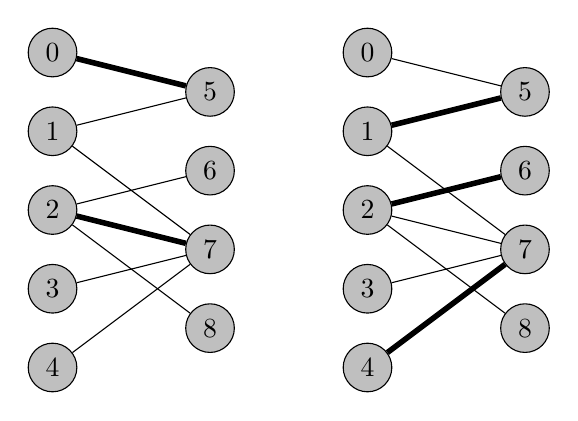
\begin{tikzpicture}[scale=1, vertex/.style = {circle,fill=gray!50,draw}, edge1/.style = {-}, edge2/.style = {-,line width=2pt}]
% vertex
\node[vertex] (n0) at (1,5)  {0};
\node[vertex] (n1) at (1,4)  {1};
\node[vertex] (n2) at (1,3)  {2};
\node[vertex] (n3) at (1,2)  {3};
\node[vertex] (n4) at (1,1)  {4};
\node[vertex] (n5) at (3,4.5)  {5};
\node[vertex] (n6) at (3,3.5)  {6};
\node[vertex] (n7) at (3,2.5)  {7};
\node[vertex] (n8) at (3,1.5)  {8};
%edges
\draw[edge1] (n1) to (n5);
\draw[edge1] (n1) to (n7);
\draw[edge1] (n2) to (n6);
\draw[edge1] (n2) to (n8);
\draw[edge1] (n3) to (n7);
\draw[edge1] (n4) to (n7);
\draw[edge2] (n0) to (n5);
\draw[edge2] (n2) to (n7);
% vertex
\node[vertex] (n10) at (5,5)  {0};
\node[vertex] (n11) at (5,4)  {1};
\node[vertex] (n12) at (5,3)  {2};
\node[vertex] (n13) at (5,2)  {3};
\node[vertex] (n14) at (5,1)  {4};
\node[vertex] (n15) at (7,4.5)  {5};
\node[vertex] (n16) at (7,3.5)  {6};
\node[vertex] (n17) at (7,2.5)  {7};
\node[vertex] (n18) at (7,1.5)  {8};
%edges
\draw[edge1] (n10) to (n15);
\draw[edge1] (n11) to (n17);
\draw[edge1] (n12) to (n17);
\draw[edge1] (n12) to (n18);
\draw[edge1] (n13) to (n17);
\draw[edge2] (n11) to (n15);
\draw[edge2] (n12) to (n16);
\draw[edge2] (n14) to (n17);
\end{tikzpicture}
\caption{Ejemplo de emparejamiento bipartito}
Un grafo bipartito $G=(V,E)$ con partición de vértices $V=L \cup R$. Un emparejamiento con cardinalidad 2, un emparejamiento máximo con cardinalidad 3. \\Fuente: \cite{Cormen2009}.
\label{empBip}
\end{figure}

\subsection{Algoritmo de Hopcroft-Karp}
\cite{Cormen2009} Explica que el problema de buscar un máximo emparejamiento bipartito en un grafo puede ser solucionado mediante el algoritmo de Hopcroft-Karp Karp. Los vértices que conforman a una arista se llaman puntos finales. Dado un grafo no direccionado y bipartito $G=(V,E)$, donde $V=L \cup R$ y todas las aristas tienen exactamente un punto final en $L$. Sea $M$ un emparejamiento en $G$. Un camino simple $P$ en $G$, es un camino de aumento con respecto a $M$ si comienza en un vértice no emparejado en $L$, si termina en un vértice no emparejado en $R$ y si sus aristas pertenecen alternativamente a $M$ y $E-M$. Un camino de aumento mas corto con respecto a un emparejamiento $M$ es un camino de aumento con un mínimo numero de aristas.

Dados dos conjuntos $A$ y $B$, la diferencia simétrica de $A \oplus B$ es definida como $(A-B) \cup (B-A)$. Es decir los elementos que están exactamente en uno de los dos conjuntos. Aplicando la definición de la diferencia simétrica, se tiene que si $M$ es un emparejamiento y $P$ es un camino de aumento con respecto a $M$, entonces la diferencia simétrica $M \oplus P$ es un emparejamiento y $|M \oplus P| = |M|+1$. nótese que si $P_1,P_2, \twodots ,P_k$ son vértices disjuntos de caminos de aumento con respecto a $M$, entonces la diferencia simétrica $M \oplus (P_1 \cup P_2 \cup  \twodots  P_k)$ es un emparejamiento con cardinalidad $|M|+k$. Es decir que al encontrar caminos de aumento, puede aumentar el numero emparejamientos. La implementación en pseudocódigo del algoritmo se encuentra en $\proc{Hopcroft-Karp}(G)$.

\begin{codebox}
\Procname{$\proc{Hopcroft-Karp}(G)$}
\li $M \gets \emptyset$
\li \Repeat
\li let $\mathcal{P} \gets \{P_1,P_2, \twodots ,P_k\}$ be a maximal set of vertex-disjoint
\zi shortest augmenting paths with respect to M
\li $M \gets M \oplus (P_1 \cup P_2 \cup  \twodots  P_k)$
\li \Until $\mathcal{P} \isequal \emptyset$
\li \Return $M$
\end{codebox}

\cite{Cormen2009} Explica que el algoritmo de Hopcroft-Karp encuentra el conjunto máximo de caminos de aumento en $O(\sqrt{|V|})$ iteraciones. Por lo cual la complejidad temporal del algoritmo es $O(|E|*\sqrt{|V|})$.

\section{Conceptos de programacion dinamica y algoritmos}
\subsection{Programación dinámica}
\cite{Cormen2009} Explica que la programación dinámica es un método para la resolución de problemas, el cual resuelve un problema combinando las soluciones de los subproblemas. La programación dinámica se aplica cuando los problemas se superponen, cuando los subproblemas comparten subproblemas, donde un algoritmo de programación dinámica resuelve un subproblemas solo una vez y guarda la respuesta en una tabla, de esta forma evita el trabajo de volver a calcular la respuesta. La programación dinámica se aplica a problema de optimización dichos problemas pueden tener mas de una solución posible, en el cual se desea encontrar el máximo o mínimo, a estas soluciones se llaman solución optima.\\

\noindent Para desarrollar un algoritmo de programación de dinámica se sigue la siguiente secuencia de pasos:
\begin{enumerate}
    \item Caracterizar la estructura de solución optima.
    \item Definir recursivamente el valor de una solución optima.
    \item Calcular el valor de una solución optima, normalmente en forma ascendente.
    \item Construir una solución optima a partir de la información calculada.
\end{enumerate}

%\subsection{El problema de la alineación de cadenas}
%\cite{Cormen2009} Explica que el problema de la alineación de cadenas o distancia de edición, consiste en dadas dos cadenas $A=[1 \twodots n]$ y $B=[1 \twodots m]$, y un conjunto de costos de operaciones de transformación. La distancia de edición de $A$ a $B$ es el costo de la secuencia de operaciones menos costosa que transforma $A$ en $B$, las operaciones se realizan en los caracteres de la cadena, que consisten en insertar, reemplazar y eliminar. Es decir, la distancia de edición es una forma de medir que tan diferentes son dos cadenas entre si.

%\subsection{Algoritmo de Needleman-Wunsch}
%\cite{Halim2019} Explica que el problema de la alineación de cadenas con operaciones de insertar, reemplazar y eliminar caracteres, puede ser solucionado mediante el algoritmo de programación dinámica de Needleman-Wunsch. Consideremos dos cadenas $A[1 \twodots n]$, $B[1 \twodots m]$. Los costos  operaciones en los caracteres $A[i]$ y $B[i]$ son los siguientes:

%\begin{enumerate}
  %\item Si los caracteres $A[i]$ y $B[i]$ coinciden, la operación puntuá $+2$.
  %\item Si los caracteres $A[i]$ y $B[i]$ no coinciden, reemplazar $A[i]$ con $B[i]$, la operación puntua $-1$.
  %\item Si se inserta un carácter en $A[i]$, la operación puntuá $-1$.
  %\item Si se elimina un carácter en $A[i]$, la operación puntuá $-1$.
%\end{enumerate}

%Se define a $V(i,j)$ como la puntuación de la alineación optima, para los prefijos $A[1 \twodots i]$ y $B[1 \twodots j]$ y $score(C1,C2)$ como la función que devuelve la puntuación, si el carácter $C1$ está alineado con el carácter $C2$.\\

%\noindent Casos base:
%\begin{itemize}
  %\item $V(0,0)=0$ \\Dos cadenas vaciás no puntúan.
  %\item $V(i,0)=i \times score(A[i],\_)$ \\Eliminar la subcadena $A[1 \twodots i]$ para realizar la alineación, $i>0$.
  %\item $V(0,j)=j \times score(\_,B[j])$ \\ Insertar espacios en $B[1 \twodots j]$ para realizar la alineación, $j>0$.
%\end{itemize}

%\noindent Recurrencias: Para $i>0$ y $j>0$:
%\begin{itemize}
  %\item $V(i,j) = max(opcion1, opcion2, opcion3)$, donde:
  %\begin{itemize}
    %\item $opcion1=V(i-1,j-1)+score(A[i],B[j])$ \\ Puntuación de coincidencia o no coincidencia.
    %\item $opcion2=V(i-1,j)+score(A[i],\_)$ \\ Eliminar $A_i$
    %\item $opcion3=V(i,j-1)+score(\_,B[j])$ \\ Eliminar $B_j$
  %\end{itemize}
%\end{itemize}

%El algoritmo de DP se concentra en tres posibilidades del ultimo par de caracteres, que deben ser una coincidencia o no coincidencia, una eliminación o una inserción. Probando todas las posibilidades, evitando recalcular los subproblemas superpuestos. Con una función de puntuación sencilla, donde una conciencia obtiene $+2$ puntos y una no coincidencia, una inserción o una eliminación obtienen $-1$ puntos, se muestra el detalle de la puntuación de alineación de A=``ACAATCC'' y B=``AGCATGC'' en la figura \ref{editDis}. Inicialmente, solo se conocen los casos base. Después, se rellenan los valores fila por fila, de izquierda a derecha. Para rellenar $V(i,j)$ para $i,j>0$, unicamente necesitamos otros tres valores: $V(i-1,j-1)$, $V(i-1,j)$ y $V(i,j-1)$. La puntuación de la alineación máxima se almacena en la celda inferior derecha.

%\begin{figure}[!h]
%\centering
%\begin{tikzpicture}[
%table/.style={
    %matrix of nodes,
    %row sep=-\pgflinewidth,
    %column sep=-\pgflinewidth,
    %nodes={rectangle,text width=1.5em,align=center,draw},
    %text depth=1.2ex,
    %text height=2ex,
    %nodes in empty cells,
%}
%]
        %\matrix (mat) [table]{
        %&\_&A&G&C&A&T&G&C\\
        %\_&0&-1&-2&-3&-4&-5&-6&-7\\
        %A&-1&2&1&0&-1&-2&-3&-4\\
        %C&-2&1&1&3&2&1&0&-1\\
        %A&-3&0&0&2&5&4&3&2\\
        %A&-4&-1&-1&1&4&4&3&2\\
        %T&-5&-2&-2&0&3&6&5&4\\
        %C&-6&-3&-3&0&2&5&5&7\\
        %C&-7&-4&-4&-1&1&4&4&7\\
    %};
    %\fill[black,opacity=0.2] (mat-2-2.north west) rectangle (mat-2-2.south east);
    %\fill[black,opacity=0.2] (mat-3-3.north west) rectangle (mat-3-3.south east);
    %\fill[black,opacity=0.2] (mat-3-4.north west) rectangle (mat-3-4.south east);
    %\fill[black,opacity=0.2] (mat-4-5.north west) rectangle (mat-4-5.south east);
    %\fill[black,opacity=0.2] (mat-5-6.north west) rectangle (mat-5-6.south east);
    %\fill[black,opacity=0.2] (mat-6-6.north west) rectangle (mat-6-6.south east);
    %\fill[black,opacity=0.2] (mat-7-7.north west) rectangle (mat-7-7.south east);
    %\fill[black,opacity=0.2] (mat-8-8.north west) rectangle (mat-8-8.south east);
    %\fill[black,opacity=0.2] (mat-9-9.north west) rectangle (mat-9-9.south east);
    %\foreach \x in {1,2,3,4,5,6,7,8,9}
    %{
        %\draw
        %([xshift=-.125\pgflinewidth]mat-\x-1.north west) --
        %([xshift=-.125\pgflinewidth]mat-\x-9.north east);
    %}
    %\draw
        %([xshift=-.125\pgflinewidth]mat-9-1.south west) --
        %([xshift=-.125\pgflinewidth]mat-9-9.south east);
    %\foreach \y in {1,2,3,4,5,6,7,8,9}
    %{
        %\draw
        %([yshift=.5\pgflinewidth]mat-1-\y.north east) --
        %([yshift=.5\pgflinewidth]mat-9-\y.south east);
    %}
    %\draw
        %([xshift=-.125\pgflinewidth]mat-1-1.north west) --
        %([xshift=-.125\pgflinewidth]mat-9-1.south west);
    %\begin{scope}[shorten >=7pt,shorten <= 7pt]
    %\draw[->,line width=1pt]  (mat-9-9.center) -- (mat-8-8.center);
    %\draw[->,line width=1pt]  (mat-8-8.center) -- (mat-7-7.center);
    %\draw[->,line width=1pt]  (mat-7-7.center) -- (mat-6-6.center);
    %\draw[->,line width=1pt]  (mat-6-6.center) -- (mat-5-6.center);
    %\draw[->,line width=1pt]  (mat-5-6.center) -- (mat-4-5.center);
    %\draw[->,line width=1pt]  (mat-4-5.center) -- (mat-3-4.center);
    %\draw[->,line width=1pt]  (mat-3-4.center) -- (mat-3-3.center);
    %\draw[->,line width=1pt]  (mat-3-3.center) -- (mat-2-2.center);
    %\end{scope}
%\end{tikzpicture}
%\caption{Ejemplo del algoritmo de Needleman-Wunsch}
%Ejemplo: A=``ACAATCC'' y B=``AGCATGC'', la puntuación de la alineación = 7. \\Fuente: \cite{Halim2019}.
%\label{editDis}
%\end{figure}

%Para evaluar la similitud entre dos cadenas, se utiliza el puntaje obtenido, el rango de puntajes esta en el intervalo $[\id{minScore} \twodots \id{maxScore}]$. En la figura \ref{intervalEdit} se muestra el rangos de puntajes.

%\begin{figure}[!h]
%\centering
%\begin{tikzpicture}[]%
    %\draw[<-] (0,0) -- (1.5,0);
    %\draw[{[-|}] (1.5,0) node[label=below:{minScore}] {} -- (3,0) node[label=below:{0}] {};
    %\draw[{|-|}] (3,0) node[label=below:{}] {} -- (4.5,0) node[label=below:{}] {};
    %\draw[{|-|}] (4.5,0) node[label=below:{}] {} -- (6,0) node[label=below:{}] {};
    %\draw[{|-]}] (6,0) node[label=below:{}] {} -- (7.5,0) node[label=below:{maxScore}] {};
    %\draw[->] (7.5,0) -- (9,0);
%\end{tikzpicture}
%\caption{Rango de puntajes Needleman-Wunsch}
%Fuente: Elaboracion propia.
%\label{intervalEdit}
%\end{figure}

%\begin{itemize}
  %\item El puntaje más alto que se puede obtener es $\id{maxScore} = 2 * \proc{max}(|A|,|B|)$. Este puntaje representa que ambas cadenas son exactamente iguales y no se utilizaron operaciones para transformar \id{A} en \id{B}.
  %\item El puntaje más bajo que se puede obtener es $\id{minScore} = -1 * \proc{max}(|A|,|B|)$. Este puntaje representa que ambas cadenas son distintas y se utilizaron varias operaciones para transformar \id{A} en \id{B}.
%\end{itemize}

%En $\proc{NEEDLEMAN-WUNSCH}(A,B)$ se tiene la implementación en pseudocódigo del algoritmo.

%\begin{codebox}
%\Procname{$\proc{NEEDLEMAN-WUNSCH}(A,B)$}
%\li $\id{n} \gets A.length$
%\li $\id{m} \gets B.length$
%\li let $T[1 \twodots n, 1 \twodots m]$ be new table
%\li \For $i \gets 1$ \To $n$
%\li \Do \For $j \gets 1$ \To $m$
%\li \Do $T[i][j] \gets 0$ \End \End
%\li \For $i \gets 1$ \To $n$
%\li \Do $T[i][0] \gets i * -1$
%\li $T[0][i] \gets i * -1$ \End
%\li \For $i \gets 1$ \To $n$
%\li \Do \For $j \gets 1$ \To $m$
%\li \Do \If $A[i-1] \isequal B[j-1]$
%\li \Then $table[i][j] \gets table[i - 1][j - 1] + 2$
%\li \Else
%\li $table[i][j] \gets table[i - 1][j - 1] - 1$ \End
%\li $table[i][j] \gets \proc{max}(table[i][j],table[i-1][j]-1)$
%\li $table[i][j] \gets \proc{max}(table[i][j],table[i][j-1]-1)$ \End \End
%\li \Return $T[n][m]$
%\end{codebox}
%La complejidad espacial de este algoritmo de DP es $O(n * m)$ el tamaño de la tabla de DP. Debemos rellenar las celdas en $O(1)$ por tanto la complejidad temporal es de $O(n * m)$.

%\subsection{Conjuntos Disjuntos}
%En \cite{Cormen2009} obtenemos una la definición de conjuntos disjuntos y la estructura de datos para conjuntos disjuntos.

%Los conjuntos disjuntos es una colección representada por $S=\{ S_1,S_2, \twodots ,S_k \}$ donde cada elemento $S_i$ representa un conjunto dinámico, y para cada elemento de la colección se cumple que $S_i \cap S_j = \emptyset$.

%La estructura de datos para conjuntos disjuntos soporta eficientemente las operaciones de crear un conjunto, búsqueda del representante de un conjunto y la unión de conjuntos.

%\noindent Sean u y v elementos de un conjunto:
%\begin{itemize}
%    \item $MAKE-SET(u)$ Crea un nuevo conjunto cuyo único miembro es u. Dado que los conjuntos son disjuntos, es necesario que u no se encuentre en otro conjunto.
%    \item $UNION(u, v)$ Une los conjuntos dinámicos que contienen a u y v, es decir $S_u \cap S_v$, el representante del conjunto resultante sera cualquiera de los dos.
%    \item $FIND-SET(u)$ devuelve un puntero al representante del conjunto que contiene a u.
%\end{itemize}

%\subsection{Detección léxica}
%Las técnicas y herramientas para computar las diferencias textuales entre documentos son bien conocidas y aprobadas. Sin embargo, las herramientas existentes como GNU diff tratan con información plana, en lugar de jerárquica. Por lo general, calculan una lista de líneas que deben cambiarse, insertarse o eliminarse para que un primer documento coincida con el segundo. \cite{ChangeDistiller}.

%\subsection{El algoritmo de Levenshtein}
\subsection{El problema de la subsecuencia comun mas larga}
La subsecuencia comun mas larga tambien es conocida por sus siglas en ingles como \id{LCS}. En \cite{Cormen2009} encontramos las siguientes definiciones. Dada una secuencia $\id{X} = [x_1, x_2, \twodots, x_m]$, una secuencia $\id{Z} = [z_1, z_2, \twodots, z_k]$ es una subsecuencia de \id{X} si existe una secuencia estrictamente creciente $[i_1,i_2,\twodots,i_k]$ de indices de \id{X} talque para todo $j=1,2,\twodots,k$ se tiene que $x_i = z_j$. Dadas dos secuencias \id{X} y \id{Y}, se dice que una secuencia \id{Z} es una subsecuencia comun de \id{X} y \id{Y} si \id{Z} es una subsecuencia de \id{X} y \id{Y}. Apartir las definiciones, el problema de la subsecuencia comun mas larga se define como: Dadas dos secuencias $\id{X} =[x_1, x_2, \twodots, x_m]$ y $\id{Y} = [y_1, y_2, \twodots, y_n]$ se desea encontrar la subsecuencia comun de longitud maxima de \id{X} y \id{Y}.

\subsection{Caracterizacion de la LCS}
Dada una secuencia $\id{X} = [x_1, x_2, \twodots, x_m]$, se define como el i-ésimo prefijo de \id{X}, para $i=1,2,\twodots,m$ como $X_i=[x_1,x_2,\twodots,x_i]$. A continuación se muestra el teorema para la subestructura optima de la subsecuencia comun mas larga:

\begin{theorem}[Subestructura optima de una LCS]\ \\
\label{LCS}
Dadas las secuencias $\id{X}=[x_1,x_2,\twodots,x_m]$ y $\id{Y}=[y_1,y_2,\twodots,y_n]$, y dado $\id{Z}=[z_1,z_2,\twodots,z_k]$ como alguna \id{LCS} de \id{X} y \id{Y}.
\begin{enumerate}
    \item Si $x_m = y_n$, entonces $z_k = x_m = y_n$ y $\id{Z}_{k-1}$ es una \id{LCS} de $\id{X}_{m-1}$ y $\id{Y}_{n-1}$.
    \item Si $x_m \neq y_n$, entonces $z_k \neq x_m$ implica que \id{Z} es una \id{LCS} de $\id{X}_{m-1}$ y \id{Y}.
    \item Si $x_m \neq y_n$, entonces $z_k \neq y_n$ implica que \id{Z} es una \id{LCS} de \id{X} y $\id{Y}_{n-1}$.
\end{enumerate}
\end{theorem}

Apartir del Teorema \ref{LCS}, se muestra que la \id{LCS} de dos secuencias contiene dentro de ella una \id{LCS} de prefijos de las dos secuencias. Por lo cual, el problema de la \id{LCS} tiene: Propiedad de subestructura optima, solución recursiva y propiedad de superposicion de subproblemas.

\subsection{Solucion recursiva de la LCS}
El teorema \ref{LCS} implica que se debe examinar uno o dos subproblemas cuando se encuentra una \id{LCS} de $\id{X} = [x_1,x_2,\twodots,x_m]$ y $\id{Y} = [y_1,y_2,\twodots,y_n]$. Si $x_m = y_n$, se debe encontrar una \id{LCS} de $\id{X}_{m-1}$ y $\id{Y}_{n-1}$. Añadiendo $x_m = y_n$ a esta \id{LCS}. Si $x_m \neq y_n$ entonces se debe resolver dos subproblemas, buscando una \id{LCS} de $\id{X}_{m-1}$ y \id{Y}, y buscando una \id{LCS} de \id{X} y $\id{Y}_{n-1}$. Cualquiera de las dos \id{LCS} que sea mas larga es un \id{LCS} de \id{X} y \id{Y}.
La propiedad de superposicion de subproblemas en el problema de la \id{LCS}. se ve al busca una \id{LCS} de \id{X} y \id{Y}, se necesita buscar la \id{LCS} de \id{X} y $\id{Y}_{n-1}$, y de $\id{X}_{m-1}$ y \id{Y}. Donde cada uno de estos subproblemas tiene el sub-subproblema de encontrar la \id{LCS} de $\id{X}_{m-1}$ y $\id{Y}_{n-1}$.

Se define a $c[i, j]$ como la longitud de una \id{LCS} de secuencias $\id{X}_{i}$ y $\id{Y}_{j}$. Si $i=0$ ó $j=0$, una de las secuencias tiene longitud cero, y por lo tanto la \id{LCS} tiene longitud cero, La subestructura optima de la \id{LCS} esta dado por la siguiente formula recursiva.

\begin{equation}
\label{eq_lcs}
c[i,j] =
     \begin{cases}
       0, \quad \text{si } i = 0 \text{ ó } j = 0\\
       c[i-1,j-1]+1, \quad \text{si } i,j > 0 \text{ y } x_i = y_j \\
       max(c[i,j-1],c[i-1,j]), \quad \text{si } i,j > 0 \text{ y } x_i \neq y_j\\
     \end{cases}
\end{equation}

En la formulacion recursiva una condicion en problema restinge cual subproblema se considera. Cuando $\id{x_i} = \id{y_j}$, se debe considerar el subproblema de buscar la \id{LCS} de $\id{X}_{i-1}$ y $\id{Y}_{j-1}$, en otro caso se considera el subproblemas de buscar la \id{LCS} de $X_i$ y $Y_{j-1}$ y el subproblema de buscar la \id{LCS} de $X_{i-1}$ y $Y_j$.

\subsection{Calculo de la longitud de la LCS}
Apartir de la ecuacion \ref{eq_lcs}, se puede escribir una algoritmo de programacion dinamica que calcule la longitud de la \id{LCS} de dos secuencias en complejidad temporal de $O(n * m)$.
El procedimiento $\proc{LCS-Length}$ toma dos secuencias $\id{X} = [x_1,x_2,\twodots,x_m]$ y $\id{Y} = [y_1,y_2,\twodots,y_n]$ como entrada, y almacena los valores $c[i,j]$ en una tabla $c[0 \twodots m, 0 \twodots n]$, y calcula los valores $c[i,j]$ comenzando de la primera fila y columna y asi sucesivamente hasta llegar a la ultima fila y columna. Tambien almacena valores en una tabla $b[1 \twodots m, 1 \twodots n]$ que sirve para construir la solucion optima. El procedimiento retorna las tablas \id{b} y \id{c}, que contienen la longitud de la \id{LCS} de \id{X} y \id{Y}. Donde $c[m,n]$ contiene la longitud de la \id{LCS} de \id{X} y \id{Y}.

\begin{codebox}
\Procname{$\proc{LCS-Length}(X,Y)$}
\li $\id{m} \gets X.length$
\li $\id{n} \gets Y.length$
\li let $b[1 \twodots m, 1 \twodots n]$ and $c[0 \twodots m, 0 \twodots n]$  be new tables
\li \For $i \gets 1$ \To $m$ \Do
\li $c[i,0] \gets 0$ \End
\li \For $j \gets 0$ \To $n$ \Do
\li $c[0,j] \gets 0$ \End
\li \For $i \gets 1$ \To $m$ \Do
\li \For $j \gets 1$ \To $n$ \Do
\li \If $x_i \isequal y_j$ \Then
\li $c[i,j] \gets c[i-1,j-1]+1$
\li $b[i,j] \gets$ ``$\nwarrow$''
\li \ElseIf $c[i-1,j] \geq c[i,j-1]$ \Then
\li $c[i,j] \gets c[i-1,j]$
\li $b[i,j] \gets$ ``$\uparrow$''
\li \ElseNoIf $c[i,j] \gets c[i,j-1]$
\li $b[i,j] \gets$ ``$\leftarrow$'' \End \End \End
\li \Return $\id{c}$ and $\id{b}$
\end{codebox}

Dadas las secuencias $\id{X} = [A,B,C,B,D,A,B]$ y $\id{Y} = [B,D,C,A,B,A]$ el procedimiento $\proc{LCS-Length}$ calcula las tablas \id{b} y \id{c} donde la longitud de la LCS es $b[7,6] = 4$, las tablas se muestran en la figura \ref{tablesLcs}.

\begin{figure}[!h]
\centering
\subfloat[Tabla \id{c}]{
\label{tableLcsC}
\begin{tabular}{cccccccc}
                       & 0                      & 1                      & 2                      & 3                      & 4                      & 5                      & 6                      \\ \cline{2-8}
\multicolumn{1}{c|}{0} & \multicolumn{1}{c|}{0} & \multicolumn{1}{c|}{0} & \multicolumn{1}{c|}{0} & \multicolumn{1}{c|}{0} & \multicolumn{1}{c|}{0} & \multicolumn{1}{c|}{0} & \multicolumn{1}{c|}{0} \\ \cline{2-8}
\multicolumn{1}{c|}{1} & \multicolumn{1}{c|}{0} & \multicolumn{1}{c|}{0} & \multicolumn{1}{c|}{0} & \multicolumn{1}{c|}{0} & \multicolumn{1}{c|}{1} & \multicolumn{1}{c|}{1} & \multicolumn{1}{c|}{1} \\ \cline{2-8}
\multicolumn{1}{c|}{2} & \multicolumn{1}{c|}{0} & \multicolumn{1}{c|}{1} & \multicolumn{1}{c|}{1} & \multicolumn{1}{c|}{1} & \multicolumn{1}{c|}{1} & \multicolumn{1}{c|}{2} & \multicolumn{1}{c|}{2} \\ \cline{2-8}
\multicolumn{1}{c|}{3} & \multicolumn{1}{c|}{0} & \multicolumn{1}{c|}{1} & \multicolumn{1}{c|}{1} & \multicolumn{1}{c|}{2} & \multicolumn{1}{c|}{2} & \multicolumn{1}{c|}{2} & \multicolumn{1}{c|}{2} \\ \cline{2-8}
\multicolumn{1}{c|}{4} & \multicolumn{1}{c|}{0} & \multicolumn{1}{c|}{1} & \multicolumn{1}{c|}{1} & \multicolumn{1}{c|}{2} & \multicolumn{1}{c|}{2} & \multicolumn{1}{c|}{3} & \multicolumn{1}{c|}{3} \\ \cline{2-8}
\multicolumn{1}{c|}{5} & \multicolumn{1}{c|}{0} & \multicolumn{1}{c|}{1} & \multicolumn{1}{c|}{2} & \multicolumn{1}{c|}{2} & \multicolumn{1}{c|}{2} & \multicolumn{1}{c|}{3} & \multicolumn{1}{c|}{3} \\ \cline{2-8}
\multicolumn{1}{c|}{6} & \multicolumn{1}{c|}{0} & \multicolumn{1}{c|}{1} & \multicolumn{1}{c|}{2} & \multicolumn{1}{c|}{2} & \multicolumn{1}{c|}{3} & \multicolumn{1}{c|}{3} & \multicolumn{1}{c|}{4} \\ \cline{2-8}
\multicolumn{1}{c|}{7} & \multicolumn{1}{c|}{0} & \multicolumn{1}{c|}{1} & \multicolumn{1}{c|}{2} & \multicolumn{1}{c|}{2} & \multicolumn{1}{c|}{3} & \multicolumn{1}{c|}{4} & \multicolumn{1}{c|}{4} \\ \cline{2-8}
\end{tabular}}
\hspace{0.8cm}
\subfloat[Tabla \id{b}]{
\label{tableLcsB}
\begin{tabular}{cccccccc}
                       & 0                      & 1                      & 2                      & 3                      & 4                      & 5                      & 6                      \\ \cline{2-8}
\multicolumn{1}{c|}{0} & \multicolumn{1}{c|}{0} & \multicolumn{1}{c|}{0} & \multicolumn{1}{c|}{0} & \multicolumn{1}{c|}{0} & \multicolumn{1}{c|}{0} & \multicolumn{1}{c|}{0} & \multicolumn{1}{c|}{0} \\ \cline{2-8}
\multicolumn{1}{c|}{1} & \multicolumn{1}{c|}{0} & \multicolumn{1}{c|}{\begin{tiny}$\uparrow$\end{tiny}} & \multicolumn{1}{c|}{\begin{tiny}$\uparrow$\end{tiny}} & \multicolumn{1}{c|}{\begin{tiny}$\uparrow$\end{tiny}} & \multicolumn{1}{c|}{\begin{tiny}$\nwarrow$\end{tiny}} & \multicolumn{1}{c|}{\begin{tiny}$\leftarrow$\end{tiny}} & \multicolumn{1}{c|}{\begin{tiny}$\nwarrow$\end{tiny}} \\ \cline{2-8}
\multicolumn{1}{c|}{2} & \multicolumn{1}{c|}{0} & \multicolumn{1}{c|}{\begin{tiny}$\nwarrow$\end{tiny}} & \multicolumn{1}{c|}{\begin{tiny}$\leftarrow$\end{tiny}} & \multicolumn{1}{c|}{\begin{tiny}$\leftarrow$\end{tiny}} & \multicolumn{1}{c|}{\begin{tiny}$\uparrow$\end{tiny}} & \multicolumn{1}{c|}{\begin{tiny}$\nwarrow$\end{tiny}} & \multicolumn{1}{c|}{\begin{tiny}$\leftarrow$\end{tiny}} \\ \cline{2-8}
\multicolumn{1}{c|}{3} & \multicolumn{1}{c|}{0} & \multicolumn{1}{c|}{\begin{tiny}$\uparrow$\end{tiny}} & \multicolumn{1}{c|}{\begin{tiny}$\uparrow$\end{tiny}} & \multicolumn{1}{c|}{\begin{tiny}$\nwarrow$\end{tiny}} & \multicolumn{1}{c|}{\begin{tiny}$\leftarrow$\end{tiny}} & \multicolumn{1}{c|}{\begin{tiny}$\uparrow$\end{tiny}} & \multicolumn{1}{c|}{\begin{tiny}$\uparrow$\end{tiny}} \\ \cline{2-8}
\multicolumn{1}{c|}{4} & \multicolumn{1}{c|}{0} & \multicolumn{1}{c|}{\begin{tiny}$\nwarrow$\end{tiny}} & \multicolumn{1}{c|}{\begin{tiny}$\uparrow$\end{tiny}} & \multicolumn{1}{c|}{\begin{tiny}$\uparrow$\end{tiny}} & \multicolumn{1}{c|}{\begin{tiny}$\uparrow$\end{tiny}} & \multicolumn{1}{c|}{\begin{tiny}$\nwarrow$\end{tiny}} & \multicolumn{1}{c|}{\begin{tiny}$\leftarrow$\end{tiny}} \\ \cline{2-8}
\multicolumn{1}{c|}{5} & \multicolumn{1}{c|}{0} & \multicolumn{1}{c|}{\begin{tiny}$\uparrow$\end{tiny}} & \multicolumn{1}{c|}{\begin{tiny}$\nwarrow$\end{tiny}} & \multicolumn{1}{c|}{\begin{tiny}$\uparrow$\end{tiny}} & \multicolumn{1}{c|}{\begin{tiny}$\uparrow$\end{tiny}} & \multicolumn{1}{c|}{\begin{tiny}$\uparrow$\end{tiny}} & \multicolumn{1}{c|}{\begin{tiny}$\uparrow$\end{tiny}} \\ \cline{2-8}
\multicolumn{1}{c|}{6} & \multicolumn{1}{c|}{0} & \multicolumn{1}{c|}{\begin{tiny}$\uparrow$\end{tiny}} & \multicolumn{1}{c|}{\begin{tiny}$\uparrow$\end{tiny}} & \multicolumn{1}{c|}{\begin{tiny}$\uparrow$\end{tiny}} & \multicolumn{1}{c|}{\begin{tiny}$\nwarrow$\end{tiny}} & \multicolumn{1}{c|}{\begin{tiny}$\uparrow$\end{tiny}} & \multicolumn{1}{c|}{\begin{tiny}$\nwarrow$\end{tiny}} \\ \cline{2-8}
\multicolumn{1}{c|}{7} & \multicolumn{1}{c|}{0} & \multicolumn{1}{c|}{\begin{tiny}$\nwarrow$\end{tiny}} & \multicolumn{1}{c|}{\begin{tiny}$\uparrow$\end{tiny}} & \multicolumn{1}{c|}{\begin{tiny}$\uparrow$\end{tiny}} & \multicolumn{1}{c|}{\begin{tiny}$\uparrow$\end{tiny}} & \multicolumn{1}{c|}{\begin{tiny}$\nwarrow$\end{tiny}} & \multicolumn{1}{c|}{\begin{tiny}$\uparrow$\end{tiny}} \\ \cline{2-8}
\end{tabular}}
\caption{Tablas calculadas por el procedimiento $\proc{LCS-Length}$}
Para dos secuencias $X=[A,B,C,B,D,A,B]$ y $Y=[B,D,C,A,B,A]$, su \id{LCS} es igual a 4.
Fuente: \cite{Cormen2009}.
\label{tablesLcs}
\end{figure}


\subsection{Construccion de la LCS}
Apartir de la tabla \id{b} que retorna el procedimiento $\proc{LCS-Length}$, se construye una \id{LCS} de $\id{X}=[x_1,x_2,\twodots,x_m]$ y $\id{Y}=[y_1,y_2,\twodots,y_n]$. Comenzando en $b[m,n]$ y siguiendo las flechas, encontramos los elemenos de la \id{LCS} en orden inverso. El siguiente procedimiento recursivo imprime una \id{LCS} de \id{X} y \id{Y}. La llamada inicial del procedimiento es $\proc{Print-LCS}(b, X, X.length, Y.length)$.

\begin{codebox}
\Procname{$\proc{Print-LCS}(b,X,i,j)$}
\li \If $i \isequal 0$ or $j \isequal 0$ \Then
\li return \End
\li \If $b[i,j] \isequal$ ``$\nwarrow$'' \Then
\li $\proc{Print-LCS}(b,X,i-1,j-1)$
\li print $x_i$
\li \ElseIf $b[i,j] \isequal$ ``$\uparrow$'' \Then
\li $\proc{Print-LCS}(b,X,i-1,j)$
\li \ElseNoIf $\proc{Print-LCS}(b,X,i,j-1)$ \End
\end{codebox}

Para la tabla \id{b} de la figura \ref{tableLcsB}, este procedimiento imprime \id{BCBA}. La complejidad temporal del procedimiento $\proc{Print-LCS}$ es de $O(m + n)$.

\section{Indices de similitud}
\cite{magurran1988} explica que los indices de similitud expresan el grado en que dos muestras son semejantes por las especies presentes en ellas. Estos valores pueden obtenerse con base en datos cualitativos o cuantitativos.

\subsection{Indice de Sorensen-Dice}
El indice de Sorensen-Dice también conocido como el coeficiente de Sorencen. Es un estadístico utilizado para comparar la similitud entre dos muestras. El indice de Sorencen-Dice se define como:

\begin{equation}
S = \frac{2*|A \cap B|}{|A|+|B|}
\label{sorencen}
\end{equation}

En la ecuacion \ref{sorencen} se muestra a: $|\id{A}|$ y $|\id{B}|$ como el numero de especies en las muestras \id{A} y \id{B}, $|A \cap B|$ como el numero de especies compartidas por las muestras y \id{S} como el indice de similitud y varia entre 0 a 1. Es decir se encuentra en el rango de $[0 \twodots 1]$.

\subsection{Indice de Jaccard}
El indice de Jaccard tambien conocido como el coeficiente de Jaccard, Es un estadistico utilizado para medir el grado de similitud entre dos conjuntos. El indice de Jaccard se define como:
\begin{equation}
J = \frac{|A \cap B|}{|A \cup B|}
\label{jaccard}
\end{equation}
En la ecuacion \ref{jaccard} se muestra a: $|A \cup B|$ como el numero de especies en las muestras \id{A} y \id{B}, $|A \cap B|$ como el numero de especies compartidas por las muestras y \id{J} como el indice de similitud y varia entre 0 a 1. Es decir se encuentra en el rango de $[0 \twodots 1]$.
